\section{Introduction}

\subsection{The general reconstruction of room layouts} %Problem statement
A reconstruction of a room is the process of taking in some data from an empty room and transforming it into its 2D floor plan. The floor plan contains basic information, such as the overall shape of the room as well as the location of windows and doors. The spatial dimensions can also be noted down, including the length of a wall or the height of the room. This floor plan is useful in many applications and services, such as virtual room design or simple information gathering in a faster, more convenient way. 

The efficient and precise reconstruction of a room has been attempted numerous
times. The data in most cases is comprised of one or more images taken of the room from various spots. The process of transformation is the presented problem, for which this paper attempts to provide a general solution to. The problems lie in the shape of a given room and how variable any room really is. Given that this problem is solved and the process is complete for any room, many new applications can emerge that utilize this process and make way for new services. The floor map would be more readily available with just a few images taken of the room. This would absolve the need for the task of creating these floor plans by hand, making the process more efficient as a result.

\subsection{The problem with reconstruction of non-cuboid spaces} %Motivation
For most rooms, we can differentiate between cuboid and non-cuboid shaped instances. a cuboid room is regular and rectangular, while a non-cuboid room can have irregular, curved, or non-right-angled surfaces. These differences are presented in Figure\ref{fig:bothfigures} In the realm of cuboid shaped rooms, some progress has been made with the goal of reconstructing. However, there is need for a less restrictive and overall more general process that is able to reconstruct rooms, regardless of shape. Is there maybe a more efficient and general process for reconstruction? This is the question we put the emphasis on in this paper.

\begin{figure}[htbp]
    \centering
    \begin{subfigure}[b]{0.38\textwidth}
        \centering
        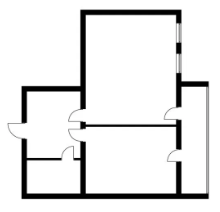
\includegraphics[width=\textwidth]{images/cuboidfloorplan.png}
        \caption{Example of cuboid rooms}
        \label{fig:cuboidroom}
    \end{subfigure}
    \hfill
    \begin{subfigure}[b]{0.38\textwidth}
        \centering
        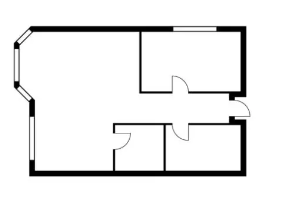
\includegraphics[width=\textwidth]{images/noncuboidfloorplan.png}
        \caption{Example of non-cuboid room (far left)}
        \label{fig:noncuboidroom}
    \end{subfigure}
    \caption{Difference in room shapes}
    \label{fig:bothfigures}
\end{figure}

This is a difficult problem for the following reasons. A room can take on different shapes, the room height can change and in some places the space can even narrow or widen. For this reason it has been proven to be a difficult challenge to efficiently map out a room's floor plan based on images. The difficulty is compounded when relying on one image to extract spatial information. Images provide limited depth perception when taken from a single viewpoint. This also makes the scaling of a processed room difficult to evaluate.

\subsection{General assumptions about space reconstruction}
When dealing with the reconstruction of spaces, there are several assumptions that are taken into account. Some assumptions may not be true for every scenario, still they remain important guiding factors in our proposed solution.
\paragraph{}

\textbf{Manhattan World Assumption} Assumes that the physical world can be represented as a series of surfaces aligned with three mutually orthogonal axes. By assuming that surfaces align with these three axes, algorithms for reconstructing 3D rooms can more easily interpret depth and geometry from 2D images, which can make reconstruction easier.

\paragraph{}

\textbf{Planar World Assumption} Assumes that the scene consists largely of planar surfaces. This assumption simplifies the reconstruction of environments by breaking down complex geometries into simpler, flat surfaces. The breaking down process remained useful as this can easily be assumed for rooms. 

\paragraph{}

\textbf{Lambertian Assumption} Assumes that surfaces reflect light uniformly in all directions, meaning that observed brightness is directly proportional to the surface orientation relative to the light source. This means that any changes in an image's luminosity is not caused by a change of light intensity, but a change in surface, texture or distance from the light source..
\paragraph{}

\textbf{Texture Consistency Assumption} Assumes that textures or colors on an object’s surface are consistent when viewed from different angles. The assumption is especially useful for detecting the same object from multiple viewpoints. It is also useful in detecting objects on a simple image, as it simplifies the detection of the object borders.

\paragraph{}

\textbf{Sparse Feature Assumption} Assumes that a reconstruction algorithm should focus on a limited number of distinct, easily identifiable points or features in the scene that can be consistently tracked across multiple images. These features are usually edges, corners or easily distingueshed areas in an image.

\subsection{Image descriptors}
This paper utilizes image descriptors. These are numerical representations of a feature on an image region. The region can be the whole image, when this is the case the descriptor is called a global descriptor. When an image region is a subset of the image, it is called a segment of the image. When a descriptor only retrieves information from a segment, it is called a local descriptor.

Descriptors can also be broken down into multiple types based on the feature they focus on. We mainly used the general information descriptors that describe one basic characteristics of an image. A characteristic can be for example color, shape or texture. During our solution we frequently relied on local descriptors that extract a single characteristic from a segment. These descriptors are also used to identify segments in a given image, like the SIFT \cite{lowe2004distinctive} and SURF \cite{speeduprobustfeatures}. The output of these two descriptors can be viewed at Figure \ref{fig:descriptoroutputs} . More information about descriptors can be found in the book Introduction to MPEG 7: Multimedia Content Description Language\cite{manjunath2002mpeg7}.

\begin{figure}[htbp]
    \centering
    \begin{subfigure}[b]{0.38\textwidth}
        \centering
        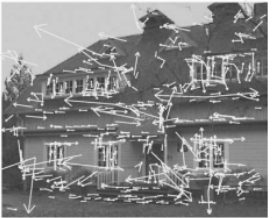
\includegraphics[width=\textwidth]{images/siftdescresult.png}
        \caption{Output of a SIFT descriptor}
        \label{fig:siftres}
    \end{subfigure}
    \hfill
    \begin{subfigure}[b]{0.38\textwidth}
        \centering
        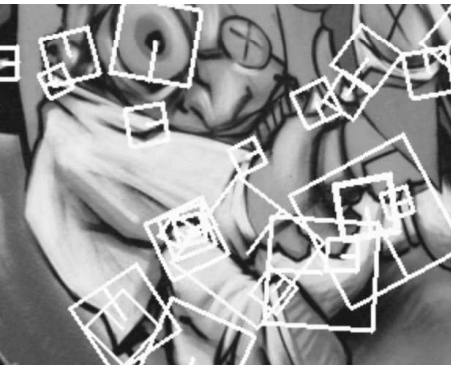
\includegraphics[width=\textwidth]{images/surfdescresult.png}
        \caption{Output of a SURF descriptor}
        \label{fig:surfres}
    \end{subfigure}
    \caption{Example of descriptors}
    \label{fig:descriptoroutputs}
\end{figure}


\subsection{The Basis of SKBD} %Solution
There are various attempts at resolving the problem of room reconstruction. Most papers in this field are concerned with the reconstruction of cuboid shaped rooms with information given from a single image. As a consequence, these results provide a limited precision on depth and scaling. The most promising papers are given more attention in Related Work[\ref{sec:relatedwork}]

Our presented solution, named Segment Knotting Boundary Detection (abbreviated to SKBD) aims to provide a more versatile method for reconstructing a room. With this paper, the aim was to develop a processing method that can reconstruct a non-cuboid shaped room from a small number of images. The solution can also determine the depth and scale properties of a room, since multiple viewpoints are being used. It also puts more emphasis on detecting segments outlined by feature points and segments detected by local descriptors. 

\subsection{Segment connection} %Contributions
This solution differs from the currently published ones in terms of usage and in terms of the reconstructing process. A heavy focus was put on image segmentation. A segment refer to a part of the image that can be detected and separated. Detecting the connection between segments involves identifying how these segments relate to one another. This could mean determining if they belong to the same structure, if they interact in some way, or if they share common features. SKBD relies on detecting segments in the taken images and then matching them. Using this approach we relied less on the proximity of these segments which in turn resulted in identifying connections that may not be immediately obvious.

%Roadmap
This article will discuss related works \ref{sec:relatedwork} in this field and how they relate to our work.  The Methodology Section \ref{sec:methodology} explains the methodology and development process of SKBD, what approaches were tried and what ultimately got implemented.
    Findings are presented in the Results Section \ref{sec:results}, where our solution is also compared to other implementations. In the Discussion Section \ref{sec:discussion} the implemented approach is discussed and in the Conclusion Section \ref{sec:conclusion} the paper is summarized. Further potential directions opened by this paper are presented in the Future Work Section \ref{sec:futurework}
